% Provenance (never printed): old seconde/premiere S material on the water
% cycle on land (the drainage basin, river discharge, floods and their
% management); see sources/book2/PROVENANCE.md. The Varden basin is computed
% in figdata/grade-10/varden_basin.py from figdata/shared/region.py; the
% Potomac record in figdata/grade-10/flood_frequency.py.
\chapter{Bassins versants, rivières et crues}\label{ch:g10:drainage-basins}

Une rivière peut monter deux jours après la fin de la pluie, dans une ville
où il n'est pas tombé une goutte. L'eau qui inonde ses rues est tombée plus
tôt, sur des collines loin en amont~; elle a dévalé leurs pentes jusqu'aux
ruisseaux, et les ruisseaux se sont réunis en la rivière qui l'a apportée,
d'un seul coup, jusqu'à la ville. Pour comprendre une crue, il faut regarder
au-delà de la rivière, vers toute la surface qui l'alimente, et y suivre
l'eau. Ce chapitre définit cette surface, le \omterm{def:g10:drainage-basins:drainage-basin}{bassin versant}~; mesure ce
qu'une rivière transporte, son \omterm{def:g10:drainage-basins:discharge}{débit}~; suit une crue à son passage en un
point de la rivière~; et montre comment un long relevé des crues indique à
quelle fréquence revient une crue donnée.

\begin{omfigure}
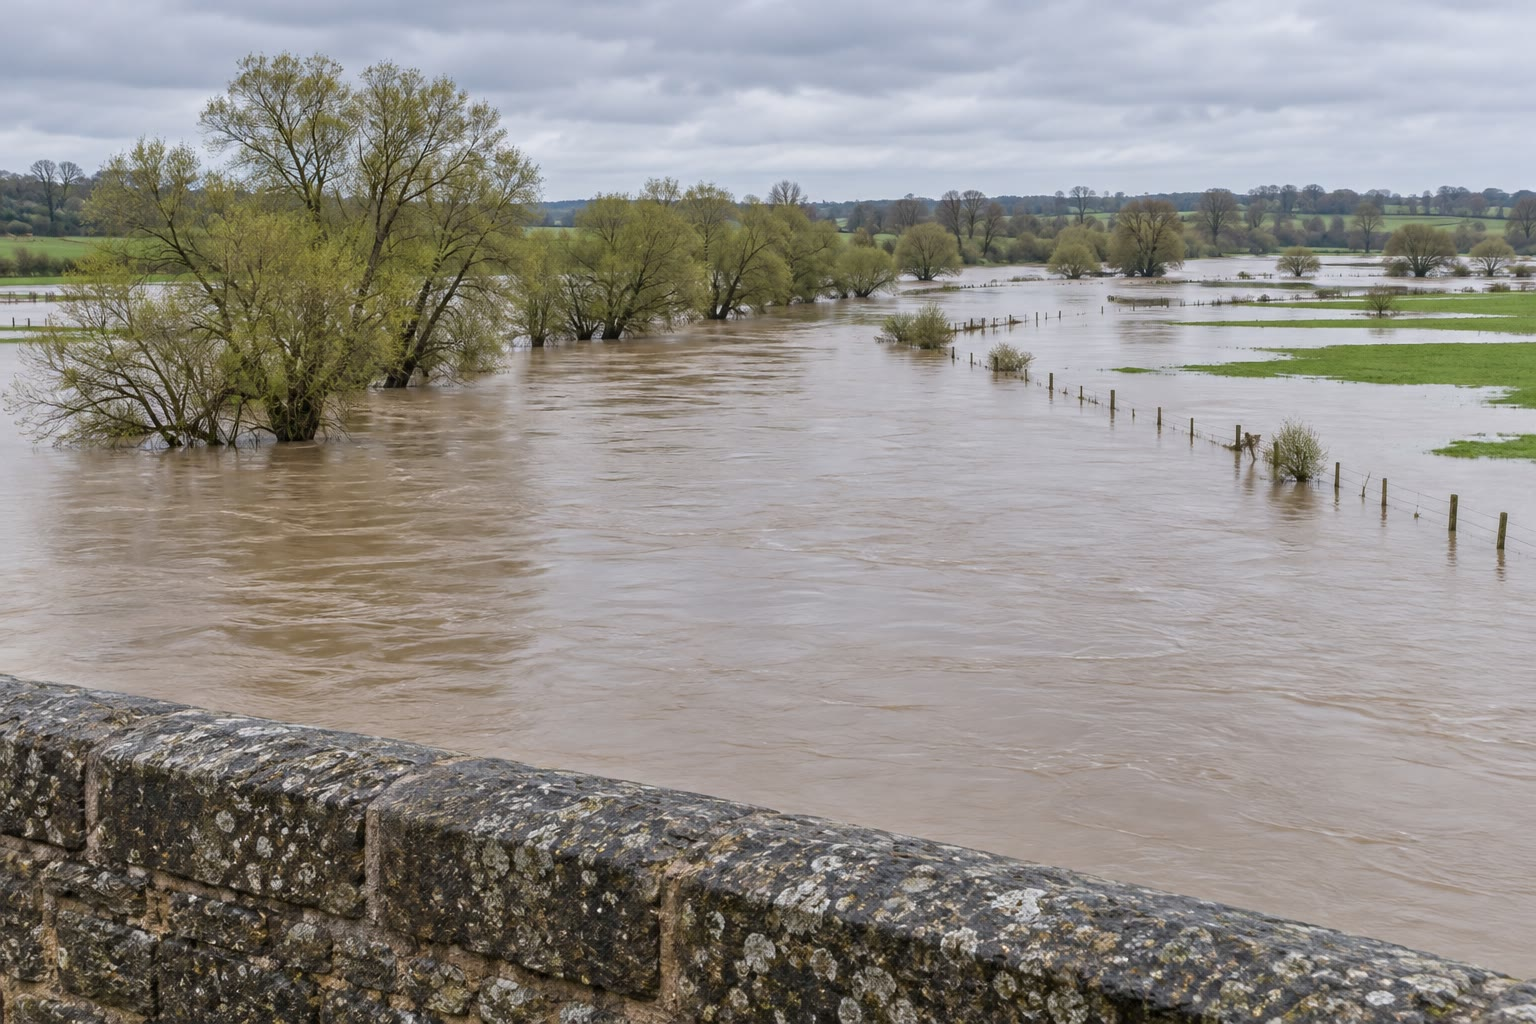
\includegraphics[width=0.8\linewidth]{images/book2/ai/g10-river-flood-meadows.jpg}

{\small Une rivière en crue, vue d'un pont de pierre~: l'eau brune, chargée
de boue, est sortie de son lit et recouvre les prés de sa plaine
d'inondation, jusqu'aux clôtures et aux arbres qui bordent ses rives
habituelles.}
\end{omfigure}

\begin{recall}
La pluie qui atteint le sol s'y infiltre, ruisselle à sa surface ou
s'évapore~; le cycle de l'eau la ramène à la mer (les livres de physique).
L'eau s'infiltre dans les roches perméables et les remplit sous la surface
de la nappe, formant des aquifères qui alimentent sources et rivières
(livre~1, année~6). Une rivière décrit des méandres dans sa plaine
d'inondation plate, qu'elle recouvre lorsqu'elle déborde (livre~1,
année~5). Les courbes de niveau joignent les points de même altitude~; les
collines de Varden sont la région dessinée sur les cartes de cette série
(livre~1, années~2 et~9).
\end{recall}

\begin{safety}
L'eau de crue est bien plus dangereuse qu'elle n'en a l'air. Environ
\qty{15}{cm} d'eau rapide peuvent renverser un adulte, et environ
\qty{30}{cm} peuvent emporter une voiture~; la route en dessous s'est
peut-être effondrée. Ne jamais marcher ni rouler dans l'eau de crue~: faire
demi-tour et prendre un autre chemin.
% ledger: nws:flood-water
\end{safety}

\section{Le bassin versant}

Toute goutte de pluie qui ne s'évapore pas ou ne s'infiltre pas en
profondeur descend la pente. Elle suit la plus grande pente du terrain,
rejoint une rigole, puis un ruisseau, et les ruisseaux se réunissent en
rivières. Toutes les terres dont l'eau aboutit à la même rivière forment une
seule unité.

\begin{definition}[Bassin versant~; ligne de partage des eaux]\label{def:g10:drainage-basins:drainage-basin}
Le \emph{bassin versant}\index{bassin versant} d'un point d'une rivière est
toute la surface de terres dont le ruissellement rejoint la rivière en amont
de ce point et passe par ce point. La
\emph{ligne de partage des eaux}\index{ligne de partage des eaux} est la ligne qui sépare deux bassins versants voisins~: elle
suit les crêtes du relief, et la pluie qui tombe de part et d'autre
s'écoule vers des rivières différentes.
\end{definition}

Un bassin est toujours défini pour un point de la rivière, son
\emph{exutoire}~: le bassin d'une rivière là où elle atteint la mer est le
plus grand, et chaque point en amont possède un bassin plus petit inclus
dans le premier. Deux gouttes tombées à un mètre l'une de l'autre, de part
et d'autre d'une ligne de partage, peuvent finir dans des rivières
différentes, et même dans des océans différents.

\subsection*{Le bassin de la rivière Varden}

Un ordinateur trouve un \omterm{def:g10:drainage-basins:drainage-basin}{bassin versant} à partir d'une carte des altitudes en
quelques étapes. La carte est découpée en petits carrés, de \qty{50}{m} de
côté ici. Pour chaque carré, l'ordinateur examine ses huit voisins et envoie
l'eau vers celui qu'on atteint par la plus forte pente descendante. (Là où
un petit creux n'a aucun voisin plus bas, on le remplit d'abord jusqu'au
niveau auquel il déborderait, comme le fait une flaque.) Suivre ces étapes
de carré en carré trace le chemin d'une goutte depuis n'importe quel point
de la carte. Les carrés dont les gouttes atteignent la rivière forment le
bassin.

\begin{omfigure}
\begin{tikzpicture}
\begin{axis}[axis equal image, xmin=0, xmax=10, ymin=0, ymax=8, width=0.86\linewidth,
  tick label style={font=\scriptsize}, xlabel={est (km)}, ylabel={nord (km)},
  label style={font=\small}, enlargelimits=false]
\addplot[fill=omDef!14, draw=none, even odd rule] table {figdata/out/grade-10-varden_basin-fill.dat};
\addplot[contour, line width=0.25pt, opacity=0.7] table {figdata/out/shared-region-contours.dat};
\addplot[index contour, opacity=0.8] table {figdata/out/shared-region-index-contours.dat};
\addplot[river, line width=1.6pt] table {figdata/out/shared-region-river.dat};
\addplot[omThm, line width=1.4pt, dashed] table {figdata/out/grade-10-varden_basin-divide.dat};
\addplot[omWxRain, line width=0.9pt, -{Stealth[length=5pt]}] table {figdata/out/grade-10-varden_basin-path1.dat};
\addplot[omWxRain, line width=0.9pt, -{Stealth[length=5pt]}] table {figdata/out/grade-10-varden_basin-path2.dat};
\addplot[omWxRain, line width=0.9pt, -{Stealth[length=5pt]}] table {figdata/out/grade-10-varden_basin-path3.dat};
\addplot[omWxRain, line width=0.9pt, -{Stealth[length=5pt]}] table {figdata/out/grade-10-varden_basin-path4.dat};
\fill[omWxRain] (axis cs:2,7.4) circle (2.2pt);
\fill[omWxRain] (axis cs:4,1.8) circle (2.2pt);
\fill[omWxRain] (axis cs:8.6,6.6) circle (2.2pt);
\fill[omWxRain] (axis cs:2.5,0.7) circle (2.2pt);
\node[font=\footnotesize, fill=white, fill opacity=0.85, text opacity=1, inner sep=1.5pt, text=omThm] at (axis cs:6.0,6.75) {ligne de partage};
\node[font=\footnotesize, fill=white, fill opacity=0.85, text opacity=1, inner sep=1.5pt, text=omThm] at (axis cs:3.5,1.1) {ligne de partage};
\node[font=\footnotesize, fill=white, fill opacity=0.85, text opacity=1, inner sep=1.5pt, align=center] at (axis cs:5.3,7.55) {hors du bassin~:\\l'eau part vers le nord};
\node[font=\footnotesize, fill=white, fill opacity=0.85, text opacity=1, inner sep=1.5pt, align=right, anchor=east] at (axis cs:9.85,3.35) {exutoire};
\draw[-{Stealth[length=6pt]}, line width=1pt, omRiver] (axis cs:9.3,3.7) -- (axis cs:9.95,4.15);
\node[font=\footnotesize, fill=white, fill opacity=0.85, text opacity=1, inner sep=1.5pt] at (axis cs:1.1,4.75) {rivière};
\end{axis}
\end{tikzpicture}

{\small Le \omterm{def:g10:drainage-basins:drainage-basin}{bassin versant} de la rivière Varden sur la carte des collines de
Varden (en grisé), calculé en envoyant l'eau de chaque carré de \qty{50}{m}
selon la plus grande pente~; courbes de niveau tous les \qty{50}{m}. Les
tirets sont les \omterm{def:g10:drainage-basins:drainage-basin}{lignes de partage des eaux}~; les lignes bleues sont les
chemins de quatre gouttes de pluie (points). Deux atteignent la rivière et
coulent vers l'est jusqu'à l'exutoire, où la rivière quitte la carte~; les
deux autres, au-delà des lignes de partage, quittent la carte vers d'autres
rivières.}
\end{omfigure}

Le bassin couvre \qty{66}{km^2} des \qty{80}{km^2} de la carte, environ les
quatre cinquièmes. Au nord, la ligne de partage suit les crêtes des collines
et passe par leurs sommets~; au-delà, le terrain descend dans la direction
opposée à la rivière et son eau s'écoule vers une autre vallée. Dans le
coin sud-ouest, une petite surface s'écoule aussi hors de la carte. La
rivière elle-même entre sur la carte par l'ouest, si bien que son bassin
complet est plus grand~: il comprend aussi les terres d'amont, au-delà du
bord de la carte.
% values computed in figdata/grade-10/varden_basin.py (basin_km2 66.19, map_km2 80)

\subsection*{Les plus grands fleuves}

On compare les fleuves par la surface de leur bassin et par l'eau qu'ils
transportent. Le plus grand fleuve du monde, de loin, est l'Amazone. Le
Mississippi, le plus grand fleuve des États-Unis, draine environ
\num{1150000}~milles carrés, soit environ 2.98~millions de \unit{km^2}, aux
États-Unis et au Canada.
% ledger: kammerer:mississippi

\section{Le débit}

\begin{definition}[Débit]\label{def:g10:drainage-basins:discharge}
Le \emph{débit}\index{debit@débit} d'une rivière en un point est le volume
d'eau qui traverse une section de la rivière en une seconde. Il se mesure en
mètres cubes par seconde, \unit{m^3/s}.
\end{definition}

Un \omterm{def:g10:drainage-basins:discharge}{débit} de \qty{1}{m^3/s} représente mille litres à chaque seconde, soit
\qty{86400}{m^3} par jour. L'eau coule le plus vite près de la surface au
milieu du chenal et le plus lentement le long du fond et des berges, contre
lesquels elle frotte~; la \emph{vitesse moyenne} est la vitesse moyennée sur
toute la section.

\begin{proposition}[Débit, vitesse et section]\label{prop:g10:drainage-basins:discharge}
Le \omterm{def:g10:drainage-basins:discharge}{débit} $Q$ d'une rivière est le produit de la vitesse moyenne $v$ de l'eau
par l'aire $A$ de la section mouillée~:
\[
Q = v\,A.
\]
\end{proposition}

\begin{proof}
Pendant une durée $t$, l'eau qui traverse la section a avancé d'une
distance $v\,t$~: elle remplit une tranche de rivière de section $A$ et de
longueur $v\,t$, de volume $A\,v\,t$. Diviser ce volume par la durée $t$
donne le volume par seconde, $Q = v\,A$.
\end{proof}

Une rivière de section \qty{50}{m^2} qui coule à une vitesse moyenne de
\qty{1.2}{m/s} transporte $1.2 \times 50 = \qty{60}{m^3/s}$. En crue, les
deux facteurs augmentent~: l'eau devient plus profonde et plus large, donc
la section grandit, et elle coule plus vite.

\subsection*{Mesurer un débit}

Comme la vitesse change d'un bord à l'autre de la rivière, on la mesure en
plusieurs points. On découpe la rivière en bandes verticales~; dans chacune,
on mesure la profondeur et la vitesse, et on additionne les \omterm{def:g10:drainage-basins:discharge}{débits} des
bandes.

\begin{method}[La méthode vitesse--surface]\label{met:g10:drainage-basins:velocity-area}
\begin{enumerate}
  \item Tendre un ruban gradué en travers de la rivière et choisir des
        verticales à intervalles réguliers $w$ le long de celui-ci.
  \item Sur chaque verticale, mesurer la profondeur $d$ et, avec un
        moulinet, la vitesse moyenne $v$ de l'eau sur cette profondeur.
  \item Chaque verticale représente une bande de largeur $w$ et d'aire
        $w\,d$~; son \omterm{def:g10:drainage-basins:discharge}{débit} vaut $v\,w\,d$.
  \item Additionner les \omterm{def:g10:drainage-basins:discharge}{débits} de toutes les bandes~: $Q = \sum v\,w\,d$.
        La section vaut $A = \sum w\,d$ et la vitesse moyenne $Q/A$.
\end{enumerate}
\end{method}

\begin{omfigure}
\begin{tikzpicture}[x=0.9cm, y=1.6cm, font=\footnotesize]
  % water
  \fill[omSea] (0,0) -- (1,-0.4) -- (2,-0.75) -- (3,-1.0) -- (4,-1.25) -- (5,-1.4) -- (6,-1.3)
     -- (7,-1.1) -- (8,-0.8) -- (9,-0.5) -- (10,-0.2) -- (10.5,0) -- cycle;
  \fill[omDef!22] (4,0) -- (4,-1.25) -- (5,-1.4) -- (6,-1.3) -- (6,0) -- cycle;
  % bed
  \draw[line width=0.9pt, brown!60!black] (-0.6,0.35) -- (0,0) -- (1,-0.4) -- (2,-0.75) -- (3,-1.0) -- (4,-1.25)
     -- (5,-1.4) -- (6,-1.3) -- (7,-1.1) -- (8,-0.8) -- (9,-0.5) -- (10,-0.2) -- (10.5,0) -- (11.1,0.35);
  \draw[omDef!70!black, line width=0.5pt] (0,0) -- (10.5,0);
  % verticals
  \foreach \x/\d/\v/\dx in {1/0.4/0.3/0.3, 3/1.0/0.6/0, 5/1.4/0.8/0, 7/1.1/0.7/0, 9/0.5/0.4/-0.25} {
    \draw[black!70, dashed] (\x,0) -- (\x,-\d);
    \node[anchor=south, font=\scriptsize] at (\x,0.02) {\qty{\v}{m/s}};
    \node[font=\scriptsize, fill=white, inner sep=0.8pt] at (\x+\dx,-0.5*\d) {\qty{\d}{m}};
  }
  \draw[{Stealth}-{Stealth}] (4,0.42) -- node[above, font=\scriptsize] {une bande~: $w = \qty{2}{m}$} (6,0.42);
  \node[anchor=west, align=left] at (11.2,-0.15) {surface\\de l'eau};
  \node[anchor=west, align=left] at (11.2,-0.9) {fond};
  \draw[black!50] (11.15,-0.9) -- (8.5,-0.68);
  \node[anchor=north] at (5.25,-1.75) {vitesses moyennes mesurées sur les verticales (au-dessus de l'eau) et profondeurs (dans l'eau)};
\end{tikzpicture}

{\small Mesure d'un \omterm{def:g10:drainage-basins:discharge}{débit} (schéma~; échelle verticale exagérée). Cinq
verticales, espacées de \qty{2}{m}, découpent en bandes un ruisseau large
d'environ \qty{10}{m}~; la bande en grisé est celle que mesure la verticale
du milieu.}
\end{omfigure}

\begin{example}[Un jaugeage]\label{ex:g10:drainage-basins:gauging}
Dans le ruisseau de la figure, les cinq bandes, larges chacune de
\qty{2}{m}, ont pour aires $2 \times 0.4 = 0.8$, $2.0$, $2.8$, $2.2$ et
\qty{1.0}{m^2}~: la section vaut \qty{8.8}{m^2}. Leurs \omterm{def:g10:drainage-basins:discharge}{débits} sont $0.3 \times 0.8 =
0.24$, $0.6 \times 2.0 = 1.20$, $0.8 \times 2.8 = 2.24$, $0.7 \times 2.2 =
1.54$ et $0.4 \times 1.0 = \qty{0.40}{m^3/s}$, si bien que le ruisseau
transporte
$Q \approx \qty{5.6}{m^3/s}$. La vitesse moyenne vaut $5.62/8.8 \approx
\qty{0.64}{m/s}$, moins que les \qty{0.8}{m/s} du milieu du ruisseau.
\end{example}

\begin{omfigure}
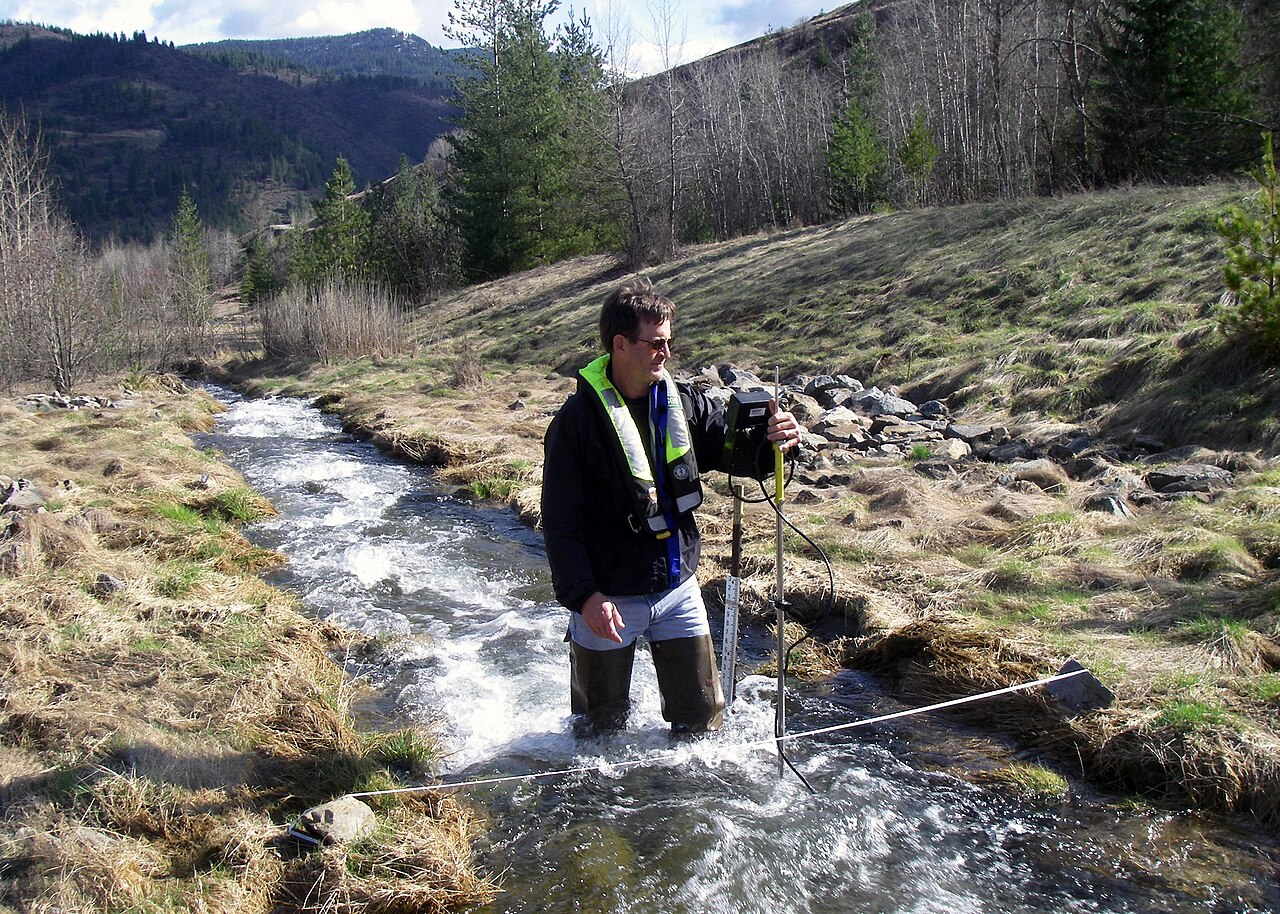
\includegraphics[height=4.6cm]{images/book2/g10-usgs-hydrologist-streamflow.jpg}\hspace{0.3cm}%
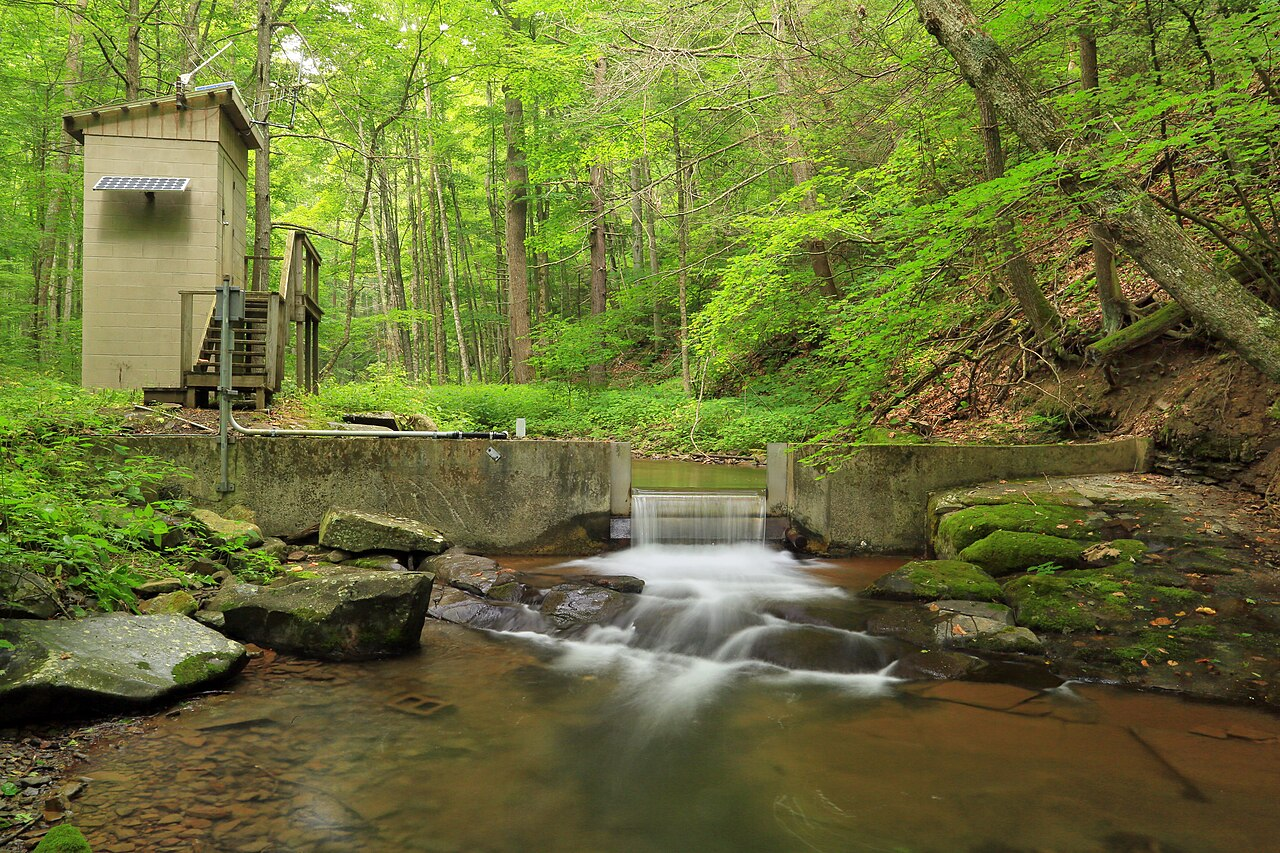
\includegraphics[height=4.6cm]{images/book2/g10-usgs-streamgage.jpg}

{\small À gauche~: une hydrologue mesure le \omterm{def:g10:drainage-basins:discharge}{débit} d'un torrent de montagne
par la méthode vitesse--surface~; le ruban tendu en travers du torrent
repère les verticales, et la perche porte un moulinet. À droite~: une
station hydrométrique sur un ruisseau forestier~; la cabane abrite les
instruments qui enregistrent le niveau de l'eau derrière le petit seuil.
Photographies~: U.S. Geological Survey (domaine public).}
\end{omfigure}

Un jaugeage prend du temps et ne peut se faire en continu. Une station
hydrométrique enregistre plutôt le niveau de l'eau, sans interruption.
Quelques jaugeages faits à différents niveaux donnent une courbe qui relie
le niveau au \omterm{def:g10:drainage-basins:discharge}{débit}, et la station convertit chaque niveau enregistré en
\omterm{def:g10:drainage-basins:discharge}{débit}.

Les grands fleuves transportent des \omterm{def:g10:drainage-basins:discharge}{débits} énormes. De 1972 à 2003,
l'Amazone a apporté à l'océan Atlantique en moyenne environ
\qty{206000}{m^3/s}, à \qty{6}{\percent} près~: environ \qty{17}{\percent}
de toute l'eau douce que les fleuves du monde apportent à la mer. Le
Mississippi apporte en moyenne \num{593000}~pieds cubes par seconde, environ
\qty{16800}{m^3/s}, au golfe du Mexique~: l'Amazone en transporte quelque
douze fois plus.
% ledger: callede:amazon, kammerer:mississippi

\section{L'hydrogramme}

\begin{definition}[Hydrogramme~; débit de base~; temps de réponse]\label{def:g10:drainage-basins:hydrograph}
Un \emph{hydrogramme}\index{hydrogramme} est le graphique du \omterm{def:g10:drainage-basins:discharge}{débit} d'une
rivière en un point en fonction du temps. Le \emph{débit de
base}\index{debit de base@débit de base} est la part du \omterm{def:g10:drainage-basins:discharge}{débit} alimentée par
les eaux souterraines, qui fait couler la rivière entre les pluies. Le
\emph{temps de réponse}\index{temps de reponse@temps de réponse} d'une crue
est la durée qui sépare le maximum de la pluie sur le bassin du maximum du
\omterm{def:g10:drainage-basins:discharge}{débit}.
\end{definition}

\begin{omfigure}
\begin{tikzpicture}[x=1cm, y=1cm, font=\footnotesize]
  \draw[-{Stealth}] (0,0) -- (10.2,0) node[below left] {temps};
  \draw[-{Stealth}] (0,0) -- (0,5.9) node[above right] {débit};
  % rain bars hanging from the top
  \draw[black!50] (0,5.4) -- (10,5.4);
  \foreach \x/\h in {1.0/0.15, 1.3/0.35, 1.6/0.55, 1.9/0.4, 2.2/0.2} {
    \fill[omWxRain!70] (\x,5.4) rectangle ++(0.28,-\h);
  }
  \node[anchor=south west] at (2.6,5.4) {pluie sur le bassin};
  % baseflow and hydrograph
  \fill[omSea] (0,0.7) -- (2.0,0.7) .. controls (2.8,0.8) and (3.3,3.3) .. (4.0,3.6)
    .. controls (4.6,3.6) and (5.1,2.1) .. (6.0,1.55) .. controls (7.0,1.0) and (8.0,0.85) .. (10,0.8)
    -- (10,0) -- (0,0) -- cycle;
  \fill[omLithAlluv] (0,0) -- (0,0.7) -- (2.0,0.7) .. controls (3.5,0.68) and (5.5,0.75) .. (6.6,0.95)
    .. controls (8,1.0) and (9,0.85) .. (10,0.8) -- (10,0) -- cycle;
  \draw[omDef, line width=1.2pt] (0,0.7) -- (2.0,0.7) .. controls (2.8,0.8) and (3.3,3.3) .. (4.0,3.6)
    .. controls (4.6,3.6) and (5.1,2.1) .. (6.0,1.55) .. controls (7.0,1.0) and (8.0,0.85) .. (10,0.8);
  \draw[black!60, dashed] (2.0,0.7) .. controls (3.5,0.68) and (5.5,0.75) .. (6.6,0.95);
  % lag time
  \draw[black!60, densely dotted] (1.74,4.85) -- (1.74,4.3);
  \draw[black!60, densely dotted] (3.98,3.65) -- (3.98,4.3);
  \draw[{Stealth}-{Stealth}] (1.74,4.3) -- node[above] {temps de réponse} (3.98,4.3);
  % labels
  \node[anchor=west] at (4.2,3.75) {pic};
  \node[anchor=east, align=right] at (2.9,2.2) {courbe\\de montée};
  \node[anchor=west, align=left] at (5.4,2.3) {courbe de décrue};
  \node[align=center] at (4.5,1.25) {ruissellement};
  \node at (8.2,0.4) {débit de base};
\end{tikzpicture}

{\small L'\omterm{def:g10:drainage-basins:hydrograph}{hydrogramme} d'une crue (schéma). Après la pluie, le \omterm{def:g10:drainage-basins:discharge}{débit} monte
jusqu'à un pic puis redescend plus lentement~; l'aire sous la courbe est le
volume d'eau. Le \omterm{def:g10:drainage-basins:hydrograph}{débit de base}, alimenté par les eaux souterraines, change
peu~; le reste est le ruissellement que la pluie a envoyé rapidement à la
rivière.}
\end{omfigure}

L'eau d'un orage atteint la rivière à des moments différents. La pluie
tombée près du chenal arrive en quelques minutes ou quelques heures~; la
pluie tombée loin en amont met bien plus longtemps, puisqu'elle doit
descendre les pentes puis suivre la rivière. Le \omterm{def:g10:drainage-basins:discharge}{débit} monte donc fortement,
sur la \emph{courbe de montée}, pendant que l'eau des pentes proches arrive,
atteint son pic quand le plus d'eau arrive à la fois, et redescend plus
lentement, sur la \emph{courbe de décrue}, à mesure que s'écoule la
dernière eau des recoins éloignés du bassin et du sol. Plus le bassin est
grand, plus le \omterm{def:g10:drainage-basins:hydrograph}{temps de réponse} est long~: quelques heures pour un petit
ruisseau, plusieurs jours pour un grand fleuve.

Certains bassins donnent des crues \emph{éclair}, avec un pic haut et
soudain et un \omterm{def:g10:drainage-basins:hydrograph}{temps de réponse} court~; d'autres donnent des crues lentes et
étalées. La même pluie donne une crue plus soudaine quand~:
\begin{itemize}
  \item le bassin est petit et pentu, si bien que l'eau a un trajet court et
        rapide~;
  \item le sol laisse peu d'eau s'infiltrer~: roche nue, argile, sol déjà
        gorgé d'eau, sol gelé, et surtout les toits, les routes et les
        parkings d'une ville, qui envoient presque toute la pluie
        directement dans les égouts et les ruisseaux~;
  \item le bassin possède un réseau dense de ruisseaux et d'égouts, qui
        collecte l'eau rapidement.
\end{itemize}
Les forêts, les sols profonds et perméables et les larges plaines
d'inondation font l'inverse~: elles retiennent l'eau et la relâchent
lentement, ce qui abaisse et retarde le pic.

\subsection*{Une crue réelle}

Le Potomac draine un bassin de \num{11560}~milles carrés, environ
\qty{29900}{km^2}, en amont d'une station hydrométrique proche de
Washington, dans l'est des États-Unis. En janvier 1996, la station a
enregistré l'\omterm{def:g10:drainage-basins:hydrograph}{hydrogramme} ci-dessous.
% ledger: data:b2-usgs-potomac

\begin{omfigure}
\begin{tikzpicture}
\begin{axis}[omrecord, width=0.86\linewidth, height=6cm, xmin=0, xmax=55, ymin=0, ymax=10000,
  xtick={0,10,20,30,40,50}, xticklabels={5 janv., 15 janv., 25 janv., 4 févr., 14 févr., 24 févr.},
  ylabel={débit (\unit{m^3/s})}, xlabel={1996},
  tick label style={font=\small}, label style={font=\small},
  scaled y ticks=false, yticklabel style={/pgf/number format/fixed}]
\addplot[omDef, line width=1.1pt, mark=*, mark size=1.1pt] table[x=day, y=q] {figdata/out/grade-10-flood_frequency-hydrograph.dat};
\node[anchor=west, font=\footnotesize] at (axis cs:17,9231) {\qty{9231}{m^3/s} le 21~janvier};
\draw[black!60, dashed] (axis cs:5,334) -- (axis cs:13,334);
\node[anchor=south, font=\footnotesize] at (axis cs:9,1000) {environ \qty{330}{m^3/s}};
\draw[black!60] (axis cs:9,1000) -- (axis cs:9,390);
\end{axis}
\end{tikzpicture}

{\small \omterm{def:g10:drainage-basins:discharge}{Débit} moyen journalier du Potomac près de Washington du 5~janvier au
29~février 1996~: la crue est passée de \qty{362}{m^3/s} le 18~janvier à
plus de \qty{9000}{m^3/s} trois jours plus tard, puis a décru au cours des
semaines suivantes, avec une seconde montée, plus faible, à la fin de
janvier. Données~: U.S. Geological Survey, station 01646500.}
\end{omfigure}
% values computed in figdata/grade-10/flood_frequency.py (hydro_peak_m3s 9231, hydro_before_mean 334)

Les jours précédant la crue, la rivière transportait environ
\qty{330}{m^3/s}, son \omterm{def:g10:drainage-basins:hydrograph}{débit de base}. Le 21~janvier, la moyenne journalière
a atteint \qty{9231}{m^3/s}, presque trente fois plus. Répartie sur tout le
bassin, l'eau passée à la station ce jour-là formerait une couche
$9231 \times 86400 / (29\,900 \times 10^6) \approx \qty{0.027}{m}$, soit
environ \qty{27}{mm} d'épaisseur~: une forte pluie, livrée en un seul jour
par tout le bassin à la fois.
% ledger: data:b2-usgs-potomac (hydro_peak_mm_per_day 26.6 in figdata/grade-10/flood_frequency.py)

\section{Les crues et leur période de retour}

Quelle crue une ville doit-elle attendre~? La réponse vient du passé~: une
station hydrométrique qui fonctionne depuis des décennies a enregistré le
plus fort \omterm{def:g10:drainage-basins:discharge}{débit} de chaque année, le \emph{pic annuel}. Les petits pics
reviennent presque chaque année, les grands rarement. Plus une crue est
rare, plus elle est forte.

\begin{definition}[Période de retour]\label{def:g10:drainage-basins:return-period}
La \emph{période de retour}\index{periode de retour@période de retour} $T$
d'une crue est l'intervalle moyen, en années, entre les années dont le pic
annuel l'égale ou la dépasse. Une crue de période de retour $T$, une
\emph{crue de $T$~ans}, a une probabilité $1/T$ d'être égalée ou dépassée
au cours d'une année quelconque.
\end{definition}

Une crue centennale n'est pas une crue qui vient une fois tous les cent ans,
comme un horaire. C'est une crue qui a une chance sur cent d'être égalée ou
dépassée chaque année, toutes les années, quoi qu'il se soit passé l'année
précédente. Deux peuvent survenir deux années de suite~; un siècle peut
passer sans aucune.

\begin{method}[Périodes de retour à partir d'un relevé de pics annuels]\label{met:g10:drainage-basins:return-periods}
\begin{enumerate}
  \item Dresser la liste des pics annuels de $n$ années.
  \item Les classer du plus grand (rang $m = 1$) au plus petit
        (rang $m = n$).
  \item Attribuer au pic de rang $m$ la \omterm{def:g10:drainage-basins:return-period}{période de retour} $T = (n + 1)/m$.
  \item Tracer les pics en fonction de $T$ sur une échelle logarithmique de
        $T$, et lire le \omterm{def:g10:drainage-basins:discharge}{débit} pour la \omterm{def:g10:drainage-basins:return-period}{période de retour} voulue.
\end{enumerate}
\end{method}

Le plus grand des $n$ pics reçoit ainsi $T = n + 1$ ans~: dans un relevé de
\num{95}~ans, \num{96}~ans. La formule traduit ce que montre le relevé~:
le pic de rang $m$ a été égalé ou dépassé au cours de $m$ des $n$ années,
environ une fois tous les $n/m$ ans. La méthode ne peut pas aller de façon
fiable au-delà de la durée du relevé~: un relevé de \num{50}~ans dit peu de
chose de la crue de \num{1000}~ans.

\begin{omfigure}
\begin{tikzpicture}
\begin{axis}[omrecord, width=0.86\linewidth, height=6.2cm, xmode=log, xmin=0.9, xmax=150,
  ymin=0, ymax=15000, xlabel={période de retour $T$ (années)}, ylabel={pic annuel (\unit{m^3/s})},
  xtick={1,2,5,10,20,50,100}, xticklabels={1,2,5,10,20,50,100},
  tick label style={font=\small}, label style={font=\small},
  scaled y ticks=false, yticklabel style={/pgf/number format/fixed}]
\addplot[only marks, mark=*, mark size=1.5pt, omDef] table[x=T, y=peak] {figdata/out/grade-10-flood_frequency-ranked.dat};
\node[anchor=east, font=\footnotesize] at (axis cs:92,13705) {1936};
\node[anchor=east, font=\footnotesize] at (axis cs:46,12658) {1942};
\node[anchor=south, font=\footnotesize] at (axis cs:32,10300) {1972};
\node[anchor=north west, font=\footnotesize, align=left] at (axis cs:1.1,14000) {Potomac près de Washington,\\pics annuels 1931--2025 ($n = 95$)};
\end{axis}
\end{tikzpicture}

{\small Les \num{95}~pics annuels du Potomac près de Washington, classés et
tracés en fonction de leur \omterm{def:g10:drainage-basins:return-period}{période de retour} $T = (n+1)/m$. Le plus grand,
en mars 1936, reçoit $T = 96$~ans. Données~: U.S. Geological Survey,
station 01646500.}
\end{omfigure}
% values computed in figdata/grade-10/flood_frequency.py

\begin{dated}{2026}
Dans le relevé du Potomac près de Washington, de 1931 à 2025, les cinq plus
grands pics annuels sont survenus en mars 1936 (\qty{13700}{m^3/s}), en
octobre 1942, en juin 1972, en avril 1937 et en janvier 1996, les deux
derniers à égalité, à \qty{9830}{m^3/s}.
% ledger: data:b2-usgs-potomac
\end{dated}

\subsection*{La probabilité d'une crue sur de nombreuses années}

Une maison ou un pont reste debout des décennies. Ce qui compte pour eux
n'est pas la probabilité d'une crue en un an, mais sur toute leur durée de
vie.

\begin{proposition}[Au moins une crue en $N$ ans]\label{prop:g10:drainage-basins:chance}
Si les années sont indépendantes les unes des autres, la probabilité qu'une
crue de \omterm{def:g10:drainage-basins:return-period}{période de retour} $T$ soit égalée ou dépassée au moins une fois en
$N$ ans vaut
\[
P = 1 - \left(1 - \frac{1}{T}\right)^{N}.
\]
\end{proposition}

\begin{proof}
En une année, la probabilité que la crue ne survienne \emph{pas} vaut
$1 - 1/T$. Les années étant indépendantes, la probabilité qu'elle ne
survienne au cours d'aucune des $N$ années est le produit de $N$ tels
facteurs, $(1 - 1/T)^N$. L'événement «~au moins une fois~» est le contraire
de «~jamais~», donc sa probabilité vaut
$1 - (1 - 1/T)^N$.
\end{proof}

Pour une crue centennale sur trente ans, $(0.99)^{30} \approx 0.740$, et
$P \approx 0.26$~: une chance sur quatre. Sur cent ans, $(0.99)^{100}
\approx 0.366$ et $P \approx 0.63$~: il est loin d'être certain que la crue
centennale survienne en cent ans.

\begin{omfigure}
\begin{tikzpicture}
\begin{axis}[omrecord, width=0.82\linewidth, height=5.8cm, xmin=0, xmax=100, ymin=0, ymax=1,
  xlabel={nombre d'années $N$}, ylabel={probabilité d'au moins une crue},
  ytick={0,0.2,0.4,0.6,0.8,1}, yticklabels={0, 20\,\%, 40\,\%, 60\,\%, 80\,\%, 100\,\%},
  tick label style={font=\small}, label style={font=\small},
  legend pos=south east, legend style={font=\footnotesize}]
\addplot[omThm, line width=1pt] table[x=n, y=p10] {figdata/out/grade-10-flood_frequency-chance.dat};
\addplot[omProp, line width=1pt] table[x=n, y=p50] {figdata/out/grade-10-flood_frequency-chance.dat};
\addplot[omDef, line width=1pt] table[x=n, y=p100] {figdata/out/grade-10-flood_frequency-chance.dat};
\legend{{crue décennale}, {crue cinquantennale}, {crue centennale}}
\draw[black!60, dashed] (axis cs:30,0) -- (axis cs:30,0.2603) -- (axis cs:0,0.2603);
\fill[omDef] (axis cs:30,0.2603) circle (2pt);
\node[anchor=north west, font=\footnotesize] at (axis cs:31,0.22) {26\,\% en 30~ans};
\end{axis}
\end{tikzpicture}

{\small La probabilité qu'une crue de \omterm{def:g10:drainage-basins:return-period}{période de retour} 10, 50 ou 100~ans
survienne au moins une fois en $N$ ans.}
\end{omfigure}
% values computed in figdata/grade-10/flood_frequency.py (chance_100_30 0.2603)

\section{Barrages et digues}

On construit depuis longtemps des ouvrages qui modifient le passage d'une
crue. Deux d'entre eux le modifient en sens opposés.

Un \emph{barrage} retient une retenue d'eau. Quand une crue arrive, une
partie de son eau est stockée dans la retenue, dont le niveau monte, puis
relâchée ensuite, sur une durée plus longue. En aval passe le même volume
d'eau, mais étalé~: le pic est plus bas et plus tardif. Une retenue n'abaisse
une crue que tant qu'il lui reste de la place~; une fois pleine, toute l'eau
qui y entre passe.

Une \emph{digue} est un remblai de terre construit le long d'une rivière
pour tenir ses crues à l'écart de la plaine d'inondation. Entre les digues,
l'eau ne peut s'étaler~; pour faire passer le même \omterm{def:g10:drainage-basins:discharge}{débit} par une section
plus étroite, elle doit monter plus haut et couler plus vite. Les terres
situées derrière les digues restent au sec, tant que les digues tiennent et
ne sont pas submergées. Mais la plaine d'inondation ne stocke plus d'eau
pendant la crue, si bien qu'une plus grande part de celle-ci descend vers
l'aval, et plus tôt.

\begin{omfigure}
\begin{tikzpicture}[x=0.62cm, y=0.62cm, font=\footnotesize]
  \begin{scope}
    \draw[-{Stealth}] (0,0) -- (9.4,0) node[below left] {temps};
    \draw[-{Stealth}] (0,0) -- (0,6.0) node[above right] {débit};
    \draw[omDef, line width=1.2pt] (0,0.6) -- (1,0.6) .. controls (1.8,0.7) and (2.2,5.2) .. (2.8,5.2)
      .. controls (3.5,5.2) and (4,1.6) .. (5,1.0) .. controls (6,0.7) and (7.5,0.6) .. (9,0.6);
    \draw[omThm, line width=1.2pt, dashed] (0,0.6) -- (1.3,0.6) .. controls (2.3,0.75) and (3.0,3.3) .. (3.8,3.3)
      .. controls (4.7,3.3) and (5.8,1.5) .. (6.8,1.0) .. controls (7.6,0.75) and (8.3,0.65) .. (9,0.6);
    \node[anchor=west, text=omDef] at (3.0,5.35) {entrée de la retenue};
    \node[anchor=west, text=omThm] at (4.2,3.55) {sous le barrage};
    \node[anchor=north] at (4.5,-0.45) {(a) un barrage~: pic plus bas et plus tardif};
  \end{scope}
  \begin{scope}[xshift=7.2cm]
    \fill[omLithAlluv] (0,0) -- (10,0) -- (10,1.8) -- (0,1.8) -- cycle;
    \fill[white] (3.5,1.8) -- (3.9,0.4) -- (6.1,0.4) -- (6.5,1.8) -- cycle;
    \fill[omSea] (0.4,2.3) -- (3.25,2.3) -- (3.5,1.8) -- (3.9,0.4) -- (6.1,0.4) -- (6.5,1.8) -- (6.75,2.3) -- (9.6,2.3) -- (9.6,1.8) -- (0.4,1.8) -- cycle;
    \draw[line width=0.8pt, brown!60!black] (0,1.8) -- (3.5,1.8) -- (3.9,0.4) -- (6.1,0.4) -- (6.5,1.8) -- (10,1.8);
    \draw[omDef!70!black] (0.4,2.3) -- (9.6,2.3);
    \node[anchor=south, text=omDef!70!black, align=center] at (1.5,2.35) {sans\\digues};
    % levees
    \fill[brown!45] (2.6,1.8) -- (3.0,3.9) -- (3.3,3.9) -- (3.5,1.8) -- cycle;
    \fill[brown!45] (6.5,1.8) -- (6.7,3.9) -- (7.0,3.9) -- (7.4,1.8) -- cycle;
    \fill[omSea!70!omDef] (3.5,1.8) -- (3.9,0.4) -- (6.1,0.4) -- (6.5,1.8) -- (6.65,3.4) -- (3.35,3.4) -- cycle;
    \draw[omThm, line width=0.8pt, dashed] (3.35,3.4) -- (6.65,3.4);
    \node[anchor=south, text=omThm] at (5,3.95) {avec digues};
    \draw[omThm] (5,3.95) -- (5,3.45);
    \node[anchor=north] at (5,-0.45) {(b) des digues~: la crue monte plus haut};
  \end{scope}
\end{tikzpicture}

{\small Schéma. (a) Une retenue stocke une partie d'une crue et la relâche
plus tard~: sous le barrage, le pic est plus bas et arrive plus tard.
(b) Sans digues, la crue s'étale en une mince couche sur la plaine
d'inondation~; entre des digues, le même \omterm{def:g10:drainage-basins:discharge}{débit} doit passer par une section
étroite et monte bien plus haut.}
\end{omfigure}

\section{Exercices}

\begin{exercise}[$\star$]\label{exo:g10:drainage-basins:1}
Définir un \omterm{def:g10:drainage-basins:drainage-basin}{bassin versant} et une \omterm{def:g10:drainage-basins:drainage-basin}{ligne de partage des eaux}. Pourquoi deux
gouttes de pluie tombées à un mètre l'une de l'autre peuvent-elles finir
dans deux mers différentes~?
\end{exercise}

\begin{exercise}[$\star$]\label{exo:g10:drainage-basins:2}
Définir le \omterm{def:g10:drainage-basins:discharge}{débit} d'une rivière et donner son unité. Combien de litres
passent en un jour en un point d'une rivière de \omterm{def:g10:drainage-basins:discharge}{débit} \qty{1}{m^3/s}~?
\end{exercise}

\begin{exercise}[$\star$]\label{exo:g10:drainage-basins:3}
Sur l'\omterm{def:g10:drainage-basins:hydrograph}{hydrogramme} du Potomac de janvier 1996, lire le \omterm{def:g10:drainage-basins:hydrograph}{débit de base} avant la
crue, le \omterm{def:g10:drainage-basins:discharge}{débit} de pointe et sa date, ainsi que le nombre de jours qu'a duré
la montée.
\end{exercise}

\begin{exercise}[$\star$]\label{exo:g10:drainage-basins:4}
Quelle est la probabilité qu'une crue de \num{50}~ans soit égalée ou
dépassée l'an prochain~? Une crue de \num{50}~ans est survenue l'an
dernier~: est-elle moins probable cette année~?
\end{exercise}

\begin{exercise}[$\star$]\label{exo:g10:drainage-basins:5}
Le Mississippi apporte en moyenne à la mer \num{593000}~pieds cubes d'eau
par seconde (\num{1}~pied = \qty{0.3048}{m}). Convertir ce \omterm{def:g10:drainage-basins:discharge}{débit} en
\unit{m^3/s}, et le comparer aux \qty{206000}{m^3/s} de l'Amazone.
\end{exercise}

\begin{exercise}[$\star\star$]\label{exo:g10:drainage-basins:6}
Une hydrologue jauge un ruisseau avec quatre verticales espacées de
\qty{1.5}{m}. Les profondeurs sont \num{0.3}, \num{0.6}, \num{0.7} et
\qty{0.4}{m}~; les vitesses moyennes \num{0.2}, \num{0.5}, \num{0.6} et
\qty{0.3}{m/s}. Calculer la section, le \omterm{def:g10:drainage-basins:discharge}{débit} et la vitesse moyenne.
\end{exercise}

\begin{exercise}[$\star\star$]\label{exo:g10:drainage-basins:7}
Un orage déverse \qty{20}{mm} de pluie sur tout le bassin de la rivière
Varden de la carte, \qty{66}{km^2}. Quel volume d'eau cela représente-t-il~?
Si toute cette eau atteignait l'exutoire en deux jours, quel serait le \omterm{def:g10:drainage-basins:discharge}{débit}
supplémentaire moyen~?
\end{exercise}

\begin{exercise}[$\star\star$]\label{exo:g10:drainage-basins:8}
Les pics annuels d'une petite rivière sur neuf ans sont, en \unit{m^3/s}~:
\num{42}, \num{65}, \num{38}, \num{120}, \num{51}, \num{47}, \num{88},
\num{35}, \num{59}. Les classer et donner les \omterm{def:g10:drainage-basins:return-period}{périodes de retour} des trois
plus grands. Quelle est la \omterm{def:g10:drainage-basins:return-period}{période de retour} du pic médian~?
\end{exercise}

\begin{exercise}[$\star\star$]\label{exo:g10:drainage-basins:9}
Le même orage tombe sur deux bassins de même surface~: l'un pentu, couvert
par une ville, l'autre en pente douce et boisé. Esquisser leurs deux
\omterm{def:g10:drainage-basins:hydrograph}{hydrogrammes} sur les mêmes axes et expliquer les différences.
\end{exercise}

\begin{exercise}[$\star\star$]\label{exo:g10:drainage-basins:10}
Au pic du 21~janvier 1996, le Potomac transportait \qty{9231}{m^3/s} depuis
un bassin de \qty{29900}{km^2}. Quelle hauteur d'eau, répartie sur tout le
bassin, représente une journée de ce \omterm{def:g10:drainage-basins:discharge}{débit}~? Comparer au \omterm{def:g10:drainage-basins:hydrograph}{débit de base} de
\qty{330}{m^3/s}.
\end{exercise}

\begin{exercise}[$\star\star$]\label{exo:g10:drainage-basins:11}
Quelle est la probabilité qu'une crue de \num{10}~ans survienne au moins une
fois en \num{10}~ans~? Qu'elle ne survienne pas du tout pendant ces dix
ans~?
\end{exercise}

\begin{exercise}[$\star\star\star$]\label{exo:g10:drainage-basins:12}
Le \omterm{def:g10:drainage-basins:discharge}{débit} qui entre dans une retenue pendant une crue monte régulièrement de
\qty{0}{m^3/s} à \qty{1200}{m^3/s} en un jour, puis redescend régulièrement
à \qty{0}{m^3/s} en deux jours (\omterm{def:g10:drainage-basins:hydrograph}{débit de base} négligé). Quel volume la crue
apporte-t-elle~? Le barrage laisse passer au plus \qty{800}{m^3/s}, et la
retenue peut stocker \num{60}~millions de \unit{m^3}. Peut-elle retenir tout
ce qui dépasse \qty{800}{m^3/s}~?
\end{exercise}

\begin{exercise}[$\star\star\star$]\label{exo:g10:drainage-basins:13}
Une rivière large de \qty{100}{m} est pleine jusqu'à ses berges à
\qty{800}{m^3/s}, avec une vitesse de \qty{2}{m/s}. Une crue de
\qty{1200}{m^3/s} arrive.
\begin{enumerate}
  \item Sans digues, les \qty{400}{m^3/s} supplémentaires s'étalent sur une
        plaine d'inondation large de \qty{900}{m}, où ils coulent à
        \qty{0.5}{m/s}. Quelle est la profondeur de l'eau sur la plaine~?
  \item Avec des digues, toute la crue passe entre elles, à \qty{2}{m/s}.
        Quelle est la profondeur de la rivière, et de combien dépasse-t-elle
        ses berges~?
\end{enumerate}
\end{exercise}

\begin{exercise}[$\star\star\star$]\label{exo:g10:drainage-basins:14}
Quelle \omterm{def:g10:drainage-basins:return-period}{période de retour} $T$ donne à une crue une chance sur deux de
survenir au moins une fois en \num{30}~ans~?
\end{exercise}

\begin{exercise}[$\star\star\star$]\label{exo:g10:drainage-basins:15}
Une petite carte est découpée en carrés de \qty{100}{m}~; leurs altitudes en
mètres sont données ci-dessous (le nord en haut). L'eau quitte chaque carré
vers le plus bas de ses quatre voisins (nord, sud, est, ouest) s'il est plus
bas~; les carrés à \qty{34}{m} (coin nord-ouest) et à \qty{30}{m} (coin
sud-est) sont les exutoires de deux ruisseaux.
\begin{center}
\begin{tabular}{|c|c|c|c|}
\hline
34 & 38 & 46 & 50 \\ \hline
37 & 42 & 48 & 47 \\ \hline
45 & 49 & 44 & 39 \\ \hline
51 & 46 & 37 & 30 \\ \hline
\end{tabular}
\end{center}
Tracer la direction d'écoulement de chaque carré, trouver le bassin de
chaque exutoire et sa surface, et tracer la \omterm{def:g10:drainage-basins:drainage-basin}{ligne de partage des eaux}.
\end{exercise}

\section{Problème~: la crue centennale}

\begin{problem}[{Problème du week-end --- à quelle fréquence la rivière entre-t-elle en ville~?}]
\label{pb:g10:drainage-basins:1}
% ledger: data:b2-usgs-potomac (values computed in figdata/grade-10/flood_frequency.py)
Imaginons une ville sur le Potomac, juste en amont de Washington, près d'une
station hydrométrique qui enregistre chaque année le plus fort \omterm{def:g10:drainage-basins:discharge}{débit} de la
rivière depuis 1931. Les pics annuels sont représentés ci-dessous~;
l'\omterm{def:g10:drainage-basins:hydrograph}{hydrogramme} de janvier 1996 est donné dans le chapitre.

\begin{center}
\begin{tikzpicture}
\begin{axis}[omrecord, width=0.9\linewidth, height=5.4cm, ybar, bar width=1.6pt, xmin=1929, xmax=2027,
  ymin=0, ymax=15000, ylabel={pic annuel (\unit{m^3/s})}, xlabel={année},
  xtick={1930,1950,1970,1990,2010}, xticklabel style={/pgf/number format/1000 sep={}},
  tick label style={font=\small}, label style={font=\small},
  scaled y ticks=false, yticklabel style={/pgf/number format/fixed}]
\addplot[fill=omDef!70, draw=none] table[x=year, y=peak] {figdata/out/grade-10-flood_frequency-record.dat};
\draw[omThm, dashed] (axis cs:1929,9500) -- (axis cs:2027,9500);
\node[anchor=south east, font=\footnotesize, text=omThm] at (axis cs:2026,9500) {\qty{9500}{m^3/s}};
\end{axis}
\end{tikzpicture}

{\small \omterm{def:g10:drainage-basins:discharge}{Débits} des pics annuels du Potomac près de Washington, années
hydrologiques 1931--2025 (une année hydrologique va d'octobre à
septembre~: la crue d'octobre 1942 compte pour 1943).
Données~: U.S. Geological Survey, station 01646500.}
\end{center}

\medskip
\noindent\textbf{Partie I --- Le bassin et le débit.}
\begin{enumerate}
  \item Le bassin de la station couvre \num{11560}~milles carrés
        (\num{1}~mille = \qty{1.609}{km}). Convertir cette surface en
        \unit{km^2}.
  \item Quelle ligne d'une carte délimite cette surface~?
  \item Le plus grand pic, le 19~mars 1936, était de \num{484000}~pieds
        cubes par seconde. Le convertir en \unit{m^3/s} (\num{1}~pied =
        \qty{0.3048}{m}).
  \item Le pic annuel médian vaut \qty{3341}{m^3/s}. Combien de fois la
        crue de 1936 dépassait-elle la médiane~?
  \item Supposons qu'au pic de 1936 la rivière ait été large de
        \qty{400}{m} et profonde de \qty{8}{m} en moyenne à la station.
        Quelle aurait été sa vitesse moyenne~?
\end{enumerate}

\medskip
\noindent\textbf{Partie II --- Lire la crue de 1996.}
\begin{enumerate}[resume]
  \item Sur l'\omterm{def:g10:drainage-basins:hydrograph}{hydrogramme} de janvier 1996, quel était le \omterm{def:g10:drainage-basins:hydrograph}{débit de base} les
        jours précédant la crue~?
  \item Quel a été le \omterm{def:g10:drainage-basins:discharge}{débit} journalier de pointe, et quel jour~?
  \item Combien de jours a duré la montée, des \qty{362}{m^3/s} du
        18~janvier jusqu'au pic~?
  \item Quelle hauteur d'eau, rapportée à tout le bassin, le jour du pic
        a-t-il fait passer à la station~?
  \item Une seconde montée, plus faible, culmine le 29~janvier. Que
        révèle-t-elle de l'eau qui atteint le bassin~?
  \item Le \omterm{def:g10:drainage-basins:discharge}{débit} était revenu vers \qty{410}{m^3/s} le 7~février. Combien
        de temps après le pic était-ce~? Pourquoi la courbe de décrue
        dure-t-elle plus longtemps que la courbe de montée~?
\end{enumerate}

\medskip
\noindent\textbf{Partie III --- Classer les crues.}
\begin{enumerate}[resume]
  \item Le relevé compte $n = 95$ pics annuels. Quelle \omterm{def:g10:drainage-basins:return-period}{période de retour} la
        méthode attribue-t-elle au plus grand~?
  \item Le pic d'octobre 1942 (\qty{12658}{m^3/s}) est classé deuxième.
        Quelle est sa \omterm{def:g10:drainage-basins:return-period}{période de retour}~?
  \item Le pic de juin 1972 (\qty{10166}{m^3/s}) est classé troisième.
        Quelle est sa \omterm{def:g10:drainage-basins:return-period}{période de retour}~?
  \item Les crues d'avril 1937 et de janvier 1996 ont été égales
        (\qty{9826}{m^3/s}). Avec les rangs 4 et 5, quelles \omterm{def:g10:drainage-basins:return-period}{périodes de
        retour} reçoivent-elles~? Le fait de partager une valeur compte-t-il
        beaucoup ici~?
  \item Sur le diagramme en barres, compter les années dont le pic a
        dépassé \qty{9500}{m^3/s}. Estimer la probabilité d'un tel pic au
        cours d'une année quelconque, et sa \omterm{def:g10:drainage-basins:return-period}{période de retour}.
\end{enumerate}

\medskip
\noindent\textbf{Partie IV --- La probabilité d'une crue.}
\begin{enumerate}[resume]
  \item Quelle est la probabilité qu'une crue de \num{100}~ans soit égalée
        ou dépassée au cours d'une année donnée~?
  \item Quelle est la probabilité qu'elle ne le soit pas, cette année-là~?
  \item Quelle est la probabilité qu'elle ne survienne pas en \num{30}~ans,
        la durée pendant laquelle une famille peut habiter une maison au
        bord de la rivière~?
  \item Quelle est la probabilité d'au moins une crue de \num{100}~ans en
        \num{30}~ans~?
\end{enumerate}
\end{problem}
